\chapter{测量质量}\label{ch:g3:measuring-mass}

在市场上：“请来一\omterm{def:g3:measuring-mass:units}{千克}苹果！”卖家把苹果倒进托盘，
直到秤“满意”为止。顾客到底点了什么？
秤又是怎样知道该何时停下的？
有了\omterm{def:g3:levers-and-scales:lever}{杠杆}和\omterm{def:g3:levers-and-scales:scale}{天平}这些工具，
我们就可以\omterm{def:g2:measuring-length:measure}{测量}一种新的东西：\omterm{def:g3:measuring-mass:mass}{质量}。

\section{质量：物体含有多少“东西”}

\begin{definition}[质量]\label{def:g3:measuring-mass:mass}
物体的\emph{质量}\index{质量}表示它由多少“东西”组成，
东西越多，质量越大，地球拉它也越用力。
这就是为什么质量大的东西拿在手里更觉沉重，
也会把\omterm{def:g3:levers-and-scales:scale}{天平}的托盘压得更低。
\end{definition}

\begin{example}[大不等于重]\label{ex:g3:measuring-mass:bignotcheavy}
枕头大到能占满你的双臂，但你很容易就能把它抱起来。
一块比你拳头还小的石头，却让你的手腕吃力。
枕头体积大，却只装着很少的“东西”，主要是羽毛和\omterm{def:g2:air-around-us:air}{空气}；
石头体积小，却装得满满的。\omterm{def:g3:measuring-mass:mass}{质量}讲的是
\emph{所含东西的多少}，而不是占据空间的大小。（这两个概念，
以及它们之间微妙的关系，
将在以后讲\omterm{def:g1:floating-and-sinking:words}{漂浮}与\omterm{def:g1:floating-and-sinking:words}{下沉}的故事时再次相遇。）
\end{example}

\begin{definition}[克与千克]\label{def:g3:measuring-mass:units}
\omterm{def:g3:measuring-mass:mass}{质量}的\omterm{def:g2:measuring-length:measure}{单位}是\emph{克}\index{克}（记作\unit{g}）和
\emph{千克}\index{千克}（记作\unit{kg}）：
\[
\qty{1}{kg} = \qty{1000}{g}.
\]
一个回形针的\omterm{def:g3:measuring-mass:mass}{质量}约为 \qty{1}{g}；一个苹果约为
\qty{150}{g}；一盒牛奶约为 \qty{1}{kg}；你自己的\omterm{def:g3:measuring-mass:mass}{质量}约为
几十千克。与米一样，这些\omterm{def:g2:measuring-length:measure}{单位}
对地球上的每一个人都是相同的。
\end{definition}

\section{用天平称重}

\begin{method}[用砝码称重]\label{met:g3:measuring-mass:weigh}
用\omterm{def:g3:levers-and-scales:scale}{天平}和一盒标有数值的金属砝码，
\omterm{def:g2:measuring-length:measure}{测量}甜瓜的\omterm{def:g3:measuring-mass:mass}{质量}（\qty{500}{g}、\qty{200}{g}、\qty{100}{g}、
\qty{50}{g}、\dots）：
\begin{enumerate}
  \item 检查空\omterm{def:g3:levers-and-scales:scale}{天平}是否保持水平；
  \item 把甜瓜放在一个托盘里；
  \item 向另一个托盘里加砝码，先加较大的合适砝码，
        直到两托盘保持水平；
  \item 把砝码加起来：它们的总和就是甜瓜的\omterm{def:g3:measuring-mass:mass}{质量}。
\end{enumerate}
若两托盘恰好与一个\qty{500}{g}、一个\qty{200}{g}和一个
\qty{100}{g}砝码平衡，则甜瓜的\omterm{def:g3:measuring-mass:mass}{质量}为 $500 + 200 + 100 =
\qty{800}{g}$。
\end{method}

\begin{omfigure}
\begin{tikzpicture}[scale=0.85]
  \draw[thick] (5.5,0) -- (5.5,2.6);
  \draw[thick] (4.9,0) -- (6.1,0);
  \draw[very thick] (2.5,2.6) -- (8.5,2.6);
  \fill (5.5,2.6) circle (2.4pt);
  \draw[thick] (2.5,2.6) -- (2.2,1.5) (2.5,2.6) -- (2.8,1.5);
  \draw[thick] (1.9,1.5) .. controls (2.5,1.05) .. (3.1,1.5);
  \draw[thick] (8.5,2.6) -- (8.2,1.5) (8.5,2.6) -- (8.8,1.5);
  \draw[thick] (7.9,1.5) .. controls (8.5,1.05) .. (9.1,1.5);
  \draw[thick, fill=omMeth, fill opacity=0.4] (2.5,1.55) circle (0.42);
  \node[font=\footnotesize] at (2.5,1.55) {甜瓜};
  % all three marked blocks, each with its value
  \draw[thick, fill=omExo, fill opacity=0.4] (8.0,1.2) rectangle (8.55,1.7);
  \node[font=\scriptsize] at (8.28,1.45) {$500$};
  \draw[thick, fill=omExo, fill opacity=0.4] (8.6,1.2) rectangle (8.95,1.5);
  \node[font=\scriptsize] at (8.78,1.35) {$200$};
  \draw[thick, fill=omExo, fill opacity=0.4] (8.1,1.7) rectangle (8.35,1.9);
  \node[font=\scriptsize] at (8.22,1.8) {$100$};
  \node[right, font=\footnotesize, align=left] at (9.35,1.7)
    {$500 + 200 + 100$：\\\qty{800}{g}砝码};
  \node[below, font=\small] at (5.5,-0.3)
    {托盘水平：甜瓜的质量等于砝码的总和};
\end{tikzpicture}

{\small 称甜瓜：逐个加砝码，直到两托盘水平；
它们的和就是答案。}
\end{omfigure}

\begin{omfigure}
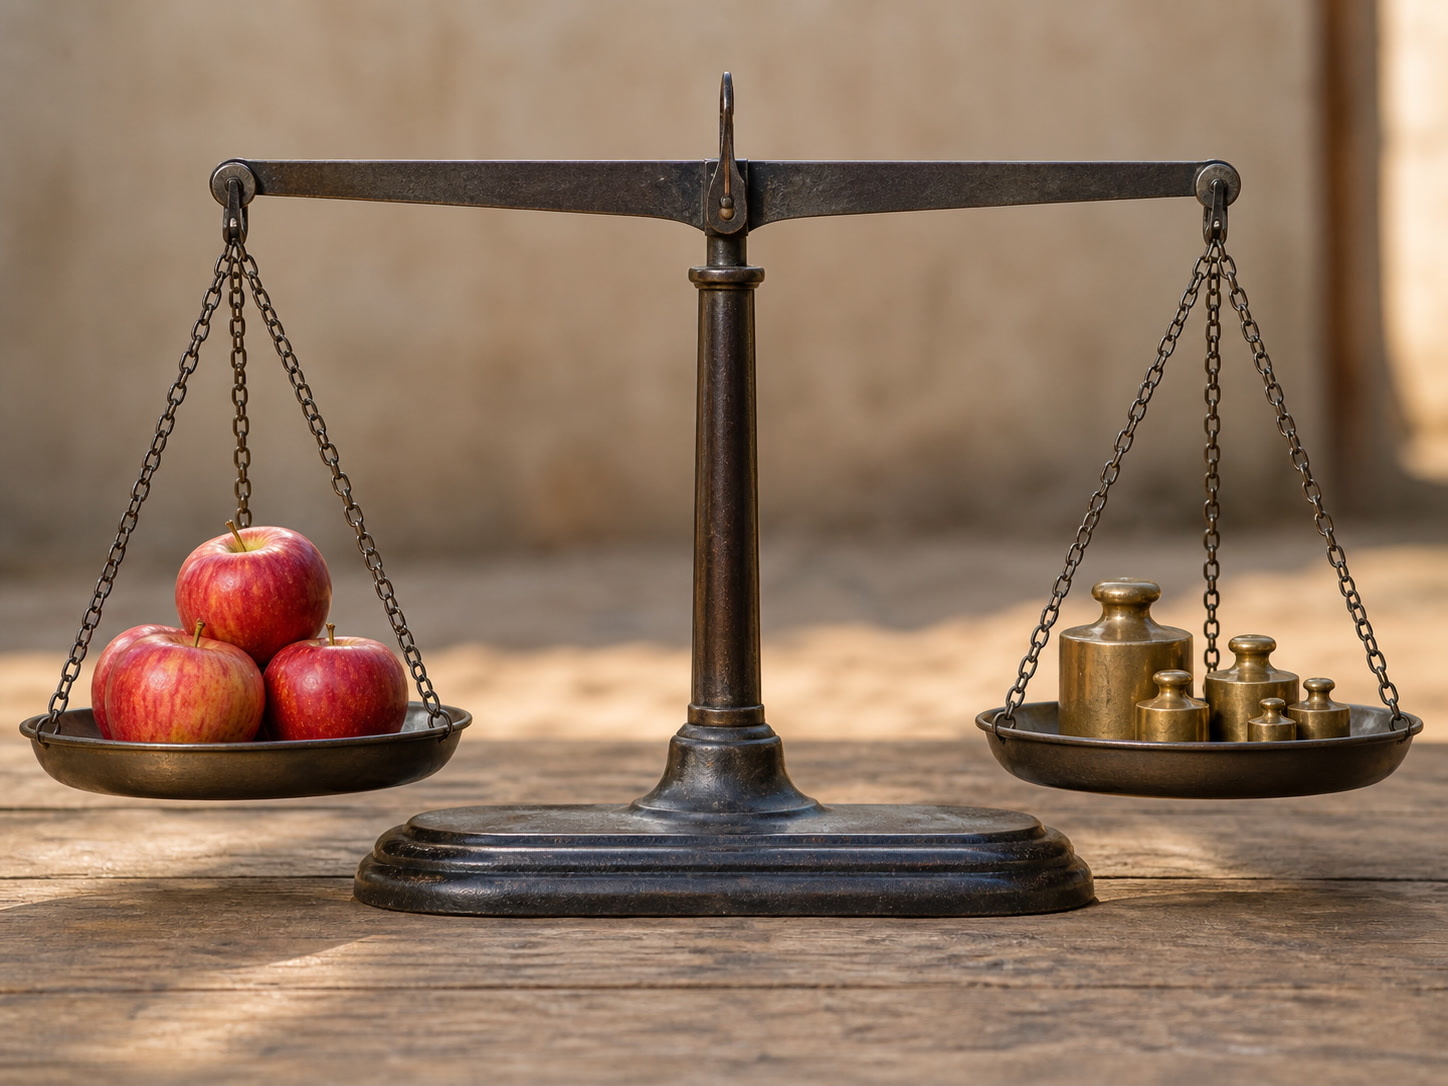
\includegraphics[width=0.52\linewidth]{images/book1/ai/g3-mass-balance-scale.jpg}

{\small \omterm{def:g3:levers-and-scales:scale}{天平}安静地工作：托盘水平，因此苹果的\omterm{def:g3:measuring-mass:mass}{质量}等于黄铜砝码的总和。}
\end{omfigure}

\begin{example}[其他的秤]\label{ex:g3:measuring-mass:otherscales}
厨房秤和浴室秤都没有第二个托盘：你把物体放上去，
指针转动（或数字亮起），直接显示
物体的\omterm{def:g3:measuring-mass:mass}{质量}。秤内有一根被压缩的弹簧替你完成比较。
方便快捷，但老式双托盘\omterm{def:g3:levers-and-scales:scale}{天平}内部没有任何隐藏的机关，
只有你已经懂得的\omterm{def:g3:levers-and-scales:lever}{杠杆}原理。
\end{example}

\begin{example}[读懂市场上的秤]\label{ex:g3:measuring-mass:market}
“一\omterm{def:g3:measuring-mass:units}{千克}苹果”的意思是：加苹果直到秤与一个
\qty{1}{kg}砝码平衡，大约是 $6$ 或 $7$ 个苹果。面粉通常装成
\qty{1}{kg}一袋，巧克力棒常常是\qty{100}{g}，一封信需要
大约 \qty{20}{g} 的纸，而邮递员的规定“不超过
\qty{20}{g}，贴一张邮票”，也是一条关于\omterm{def:g3:measuring-mass:mass}{质量}的规定。
\end{example}

\section{质量跟随“东西”的多少}

\begin{proposition}[同样的东西，质量相同]\label{prop:g3:measuring-mass:conserved}
改变东西的\emph{形状}并不改变它的\omterm{def:g3:measuring-mass:mass}{质量}。把
一团面团搓成一根长条、压成一张薄饼，或把它
切成四块后将所有碎块一起称重：秤每次显示的
\omterm{def:g3:measuring-mass:mass}{质量}都相同。\omterm{def:g3:measuring-mass:mass}{质量}计量的是东西的多少——压扁、搓长、
切开，都既不会增加东西，也不会减少东西。
\end{proposition}

\begin{omfigure}
\begin{tikzpicture}[scale=0.85]
  \draw[thick, omDef!70!black, fill=omDef, fill opacity=0.5]
    (1.3,1.0) circle (0.55);
  \node[below, font=\small, align=center] at (1.3,0.15)
    {一团面团：\\\qty{300}{g}};
  \draw[thick, omDef!70!black, fill=omDef, fill opacity=0.5]
    (6.2,0.85) ellipse (1.5 and 0.28);
  \node[below, font=\small, align=center] at (6.2,0.15)
    {搓成长条：\\\qty{300}{g}};
  \draw[thick, omDef!70!black, fill=omDef, fill opacity=0.5]
    (9.55,0.75) circle (0.3);
  \draw[thick, omDef!70!black, fill=omDef, fill opacity=0.5]
    (10.28,0.75) circle (0.3);
  \draw[thick, omDef!70!black, fill=omDef, fill opacity=0.5]
    (9.72,1.32) circle (0.28);
  \draw[thick, omDef!70!black, fill=omDef, fill opacity=0.5]
    (10.4,1.32) circle (0.28);
  \node[below, font=\small, align=center] at (10.0,0.15)
    {四块放在一起：\\\qty{300}{g}};
\end{tikzpicture}

{\small 同一团面团，三种形状，一个\omterm{def:g3:measuring-mass:mass}{质量}。
秤从不会被形状的改变所迷惑。}
\end{omfigure}

\begin{remark}[秤不看外表]\label{rem:g3:measuring-mass:appearances}
这正是\omterm{def:g2:measuring-length:measure}{测量}的无声力量：肉眼会认为压扁的薄饼
“比它原来的面团球更大”，蓬松的枕头
“比石头更重”——但\omterm{def:g3:levers-and-scales:scale}{天平}和
此前的\omterm{def:g3:temperature-thermometers:temperature}{温度计}和尺子一样，只反映东西的多少，
别无其他。我们的仪器正逐一把“看起来”的
说法换成“确实如此”。
\end{remark}

\section{练习}

\begin{exercise}[$\star$]\label{exo:g3:measuring-mass:1}
东西的\omterm{def:g3:measuring-mass:mass}{质量}说明了什么？用哪两个\omterm{def:g2:measuring-length:measure}{单位}来\omterm{def:g2:measuring-length:measure}{测量}它，
一\omterm{def:g3:measuring-mass:units}{千克}等于多少克？
\end{exercise}

\begin{exercise}[$\star$]\label{exo:g3:measuring-mass:2}
选出更合理的\omterm{def:g3:measuring-mass:mass}{质量}：一枚回形针——\qty{1}{g} 还是 \qty{1}{kg}？
一个苹果——\qty{150}{g} 还是 \qty{15}{kg}？一盒牛奶——
\qty{1}{g} 还是 \qty{1}{kg}？一只猫——\qty{4}{kg} 还是 \qty{400}{kg}？
\end{exercise}

\begin{exercise}[$\star$]\label{exo:g3:measuring-mass:3}
南瓜放在\omterm{def:g3:levers-and-scales:scale}{天平}一端，另一端放一个\qty{500}{g}的砝码和两个
\qty{200}{g}的砝码时\omterm{def:g3:levers-and-scales:scale}{天平}恰好平衡。南瓜的\omterm{def:g3:measuring-mass:mass}{质量}是多少？
\end{exercise}

\begin{exercise}[$\star$]\label{exo:g3:measuring-mass:4}
称重前，为什么空秤必须先调成水平？（想一想
那个缺斤短两的奸商。）
\end{exercise}

\begin{exercise}[$\star$]\label{exo:g3:measuring-mass:5}
沙滩球比一罐汤大得多，但这罐汤
却把秤盘压下去。请结合
\cref{ex:g3:measuring-mass:bignotcheavy}解释。
\end{exercise}

\begin{exercise}[$\star$]\label{exo:g3:measuring-mass:6}
\qty{2}{kg} 是多少克？半\omterm{def:g3:measuring-mass:units}{千克}是多少克？
哪个\omterm{def:g3:measuring-mass:mass}{质量}更大：\qty{1200}{g} 还是 \qty{1}{kg}？
\end{exercise}

\begin{exercise}[$\star$]\label{exo:g3:measuring-mass:7}
一块\qty{100}{g}的巧克力棒被掰成所有的
小方块，并把所有小方块一起放上秤。秤显示多少\omterm{def:g3:measuring-mass:mass}{质量}，
由哪条定律说明？
\end{exercise}

\begin{exercise}[$\star$]\label{exo:g3:measuring-mass:8}
厨房秤和双盘\omterm{def:g3:levers-and-scales:scale}{天平}都可以称一袋
面粉。它们各自靠什么进行比较？其中哪一种
依据你三章前学过的规律工作？
\end{exercise}

\begin{exercise}[$\star$]\label{exo:g3:measuring-mass:9}
面包师需要\qty{800}{g}面粉，手里有
\qty{500}{g}、\qty{200}{g}、\qty{200}{g}、\qty{100}{g}和
\qty{50}{g}的砝码。请找出两种不同的方法，
恰好称出\qty{800}{g}面粉——已知砝码可以放在
\emph{任一}秤盘中。
\end{exercise}

\begin{exercise}[$\star\star$]\label{exo:g3:measuring-mass:10}
尼娜称了一整个橙子：\qty{200}{g}。她剥去橙皮后单独称
去皮的橙子：\qty{160}{g}。是否
\cref{prop:g3:measuring-mass:conserved}不成立？那
缺少的克数去哪儿了？尼娜如何只再称一次就能证明？
\end{exercise}

\begin{exercise}[$\star\star$]\label{exo:g3:measuring-mass:11}
这道谜题终于对你来说不难了：一\omterm{def:g3:measuring-mass:units}{千克}羽毛和一\omterm{def:g3:measuring-mass:units}{千克}铁，
哪个\omterm{def:g3:measuring-mass:mass}{质量}更大？哪个占的空间更大？请解释
为什么那么多人会答错第一个问题。
\end{exercise}
